\chapter{Potentials}

\section{Laplace's Equation}

\subsection{Introduction}

We are interested in the differential form of Poisson's equation,
\[\nabla^2V=-\frac{\rho}{\varepsilon_0},\]
which is equivalent to the integral form
\[V(\vec{r})=\frac{1}{4\pi\varepsilon_0}\iiint\frac{\rho(\vec{r'})}{\scr}d\tau'\]
if we're given boundary conditions.

More often, we're interested in finding the potential in regions where $\rho=0$. Here, Poisson's equation reduces to Laplace's equation
\[\nabla^2V=0,\qquad\text{or}\qquad \frac{\partial^2V}{\partial x^2}+\frac{\partial^2V}{\partial y^2}+\frac{\partial^2V}{\partial z^2}=0.\]
This is so fundamental the subject that one might say electrostatics \textit{is} the study of Laplace's equation. This equation plays a role in many branches of physics and mathematics.

\begin{definition}
A solution to Laplace's equation is called a \vocab{harmonic function}.
\end{definition}

To get a feel for these harmonic functions, we will begin in lower dimensions.

\subsection{Laplace's Equation in One Dimension}

In one dimension, Laplace's equation is
\[\frac{d^2V}{dx^2}=0.\]
This means the derivative $\frac{dV}{dx}$ is constant over $x$; hence, the general solution is a straight line
\[V(x)=mx+b.\]
Since it contains two free variables, this solution is appropriate for a second-order differential equation (as we need to specify some pair of either $V$ or $V'$ as initial conditions).

There are two important features of this result that generalize nontrivially in higher dimensions:
\begin{enumerate}
    \item $V(x)$ is the \textit{average} of $V(x+a)$ and $V(x-a)$, for \textit{any} $a$:
    \[V(x)=\frac{1}{2}[V(x+a)+V(x-a)].\]
    Hence, Laplace's equation tells you to average values; if you're given some endpoints as boundary conditions, harmonic functions are, in this sense, as \textit{boring as they possibly could be} yet still fit the endpoints.
    \item Laplace's equation allows \textit{no local maxima or minima}; the only extreme values of $V$ can occur at the endpoints. This is a consequence of the above property: if there were a local maxima then it wouldn't be an average of its neighbors.
\end{enumerate}

\subsection{Laplace's Equation in Two Dimension}

In two dimensions, Laplace's equation is
\[\frac{\partial^2V}{\partial x^2}+\frac{\partial^2V}{\partial y^2}=0.\]
This is no longer an ordinary differential equation: the partial derivatives make it a \textit{partial} differential equation. Thus, some simple rules no longer apply: for example, the general solution doesn't contain two free variables (or any finite number of free variables) even though it is second order. Therefore, one cannot write down a simple ``general solution", at least not in closed form.

An example of a two-dimensional harmonic function is obtained by stretching a thin rubber sheet (or a soap film) over a support. Then, the resultant function will be roughly a harmonic function. These have the same two properties that we saw in one dimension:

\begin{enumerate}
    \item The value of $V$ at a point $(x,y)$ is the average of those \textit{around} the point: more precisely, if you draw a circle of any radius $R$ about the point $(x,y)$, then 
    \[V(x,y)=\frac{1}{2\pi R}\oint_{\text{circle}}Vd\ell.\]
    This suggests the \vocab{method of relaxation} for solving Laplace's equation given boundary conditions, which involves starting with a reasonable set of guesses then iteratively refining the guesses by averaging out points until they settle.
    \item $V$ has no local maxima or minima; all extrema occur at the boundaries. Once again, this follows from the previous property.
\end{enumerate}

\subsection{Laplace's Equation in Three Dimensions}

Now we're onto the good stuff. However, now we can offer neither an explicit solution nor a suggestive physical example. Nonetheless, the same two properties hold, and a proof will be sketched (using Coulomb's law; a proof using only Laplace's equation is given as a problem at the end of the chapter).

\begin{proposition}
The two properties hold for harmonic functions in three dimensions:
\begin{enumerate}
    \item The value of $V$ at a point $\vec{r}$ is the average of $V$ over a spherical surface of radius $R$ centered at $\vec{r}$:
    \[V(\vec{r})=\frac{1}{4\pi R^2}\oiint_{\text{sphere}}V da.\]
    \item Hence, $V$ has no local maxima or minima; the extrema must occur at boundaries.
\end{enumerate}
\end{proposition}

\begin{proof}
Let's calculate the average potential over a spherical surface of radius $R$ due to a \textit{single} point charge $q$ located outside the sphere. Place the sphere at the origin, and put $q$ on the $z$-axis, $z$ away from the center of the sphere.

Then, we can calculate the average potential across the sphere to be
\begin{align*}
    \frac{1}{4\pi R^2}\oiint_{\text{sphere}}Vda&=\frac{1}{4\pi R^2}\int_{\varphi=0}^{2\pi}\int_{\theta=0}^\pi \frac{1}{4\pi\varepsilon_0}\frac{q}{\sqrt{z^2+R^2-2zR\cos\theta}}R^2\sin\theta d\theta d\varphi\\
    &=\frac{q}{8\pi \varepsilon_0}\int_0^\pi \frac{\sin\theta}{\sqrt{z^2+R^2-2zR\cos\theta}}d\theta\\
    &=\frac{q}{8\pi\varepsilon_0}\left[-\frac{1}{zR}\cdot \sqrt{z^2+R^2-2zR\cos\theta}\right]_0^\pi\\
    &=\frac{q}{8\pi\varepsilon_0zR}\left(\sqrt{z^2+R^2-2zR}-\sqrt{z^2+R^2+2zR}\right)\\
    &=\frac{q}{4\pi\varepsilon_0z},
\end{align*}
which is exactly the electric potential at the center! By the superposition principle, the same goes for \textit{any collection} of charges outside the sphere: their average potential over the sphere is equal to the net potential they produce at the center. Note that we ignore cases where there are charges inside the sphere, since that would violate $\rho=0$.
\end{proof}

\subsection{Boundary Conditions and Uniqueness Theorems}

Laplace's equation by itself doesn't determine $V$; we need boundary conditions. But what boundary conditions are appropriate to restrict $V$ sufficiently but not cause inconsistencies?

It is clear in one dimension, but the \textit{partial} differential equations in two and three dimensions make the issue harder.  As it turns out, $V$ \textit{is} uniquely determined by its value at the boundary. However, other boundary conditions can also be used. The proof that a proposed set of boundary conditions will suffices is usually presented in the form of a \vocab{uniqueness theorem}; we do not seek to prove the \textit{existence} of solutions, but this is generally clear on physical grounds.

\begin{theorem}[First uniqueness theorem]
    The solution to Laplace's equation in some volume $\mathcal{V}$ is uniquely determined if $V$ is specified on the boundary surface $\partial\mathcal{V}$.
\end{theorem}

\begin{proof}
There is a rather clever trick to solve this problem: suppose that there exist two such solutions $V_1$ and $V_2$ such that $V_1=V_2$ on $\partial\mathcal{V}$ and $\nabla^2 V_1=\nabla^2 V_2=0$ inside $\mathcal{V}$.

The key is to \textbf{consider the difference} $V_3:=V_1-V_2$. Now, $V_3=0$ on all of $\partial \mathcal{V}$, and because of the linearity of the del operator, we have
\[\nabla^2V_3=\nabla^2 V_1-\nabla^2V_2=0\]
inside all of $\mathcal{V}$; hence $V_3$ is also a harmonic function. However, $V_3$ has no local extrema inside $\mathcal{V}$, and since it is zero on all of $\partial\mathcal{V}$, this implies that it is indeed zero inside all of $\mathcal{V}$ as well (otherwise we would be able to find some local extrema not at the boundary). Hence $V_1=V_2$, and the solution is unique.
\end{proof}

\begin{example}
Show that the potential is \textit{constant} inside an enclosure completely surrounded by conducting material, provided there is no charge within the enclosure.
\end{example}

\begin{proof}
Since it is a conductor, the boundary of the enclosure is equipotential, say at $V_0$. It is easy to see that $V=V_0$ everywhere inside is a valid solution to Laplace's equation. The first uniqueness theorem guarantees that this is the only one.
\end{proof}

It turns out the first uniqueness theorem works even if we sprinkle in some charge: the argument works the same, instead now we subtract $\nabla^2V_1=\nabla^2V_2=-\frac{\rho}{\varepsilon_0}$ to get $\nabla^2V_3=0$. In either case, the \textit{difference} $V_3:=V_1-V_2$ is a harmonic function and hence satisfies Laplace's equation with zeros on the boundary.

\begin{corollary}
The potential in a volume $\mathcal{V}$ is uniquely determined if we specify  
\begin{enumerate}[(a)]
    \item the charge density throughout the region and
    \item the values of $V$ on all boundaries.
\end{enumerate}
\end{corollary}

\subsection{Conductors and the Second Uniqueness Theorem}

If we don't know the potentials of certain conductors (by attaching them to the zero potential ground or fixed potential batteries) and instead we know the charges on conductors, do we know that there exists one unique charge distribution and therefore generated electric field? As it turns out, we do.

\begin{theorem}[Second uniqueness theorem]
    In a volume $\mathcal{V}$ surrounded by conductors and containing a specified charge density $\rho$, the electric field is uniquely determined if the \textit{total} charge on each conductor is given. (The outer boundary can be at infinity, so unbounded.)
\end{theorem}

\begin{proof}
    Once again, assume there exist two electric fields $\vec{E}_1$ and $\vec{E}_2$. We know that in the space between the conductors,
    \[\nabla\cdot \vec{E}_1=\nabla\cdot\vec{E}_2=\frac{\rho}{\varepsilon_0}.\]
    In addition, for a Gaussian surface $\mathcal{S}_i$ just enclosing the $i$th conductor with charge $Q_i$, we have that
    \[\oiint_{\mathcal{S}_i}\vec{E}_1\cdot d\vec{a}=\oiint_{\mathcal{S}_i}\vec{E}_2\cdot d\vec{a}=\frac{Q_i}{\varepsilon_0}.\]
    In addition, if we set the Gaussian surface as the outer boundary, we get
    \[\oiint_{\text{outer boundary}}=\vec{E}_1\cdot d\vec{a}=\oiint_{\text{outer boundary}}=\vec{E}_2\cdot d\vec{a}=\frac{Q_{\text{tot}}}{\varepsilon_0}.\]
    Now, we examine the difference $\vec{E}_3:=\vec{E}_1-\vec{E}_2$, which obeys 
    \[\nabla\cdot \vec{E}_3=0\]
    in the region between conductors, and
    \[\oiint\vec{E}_3\cdot d\vec{a}=0\]
    over each of the bounding surfaces $\mathcal{S}_i$ as well as the outer boundary.
    
    Finally, we exploit the fact that each conductor is an equipotential; hence $V_3$ is \textit{constant} over each conducting surface (not necessarily the same constant across different conductors). Then, invoking one of the divergence product rules (in Theorem \ref{divprodrul}), we get
    \[\nabla\cdot (V_3\vec{E}_3)=V_3(\nabla\cdot \vec{E}_3)+\vec{E}_3\cdot(\nabla V_3)=-(E_3)^2,\]
    where we use that $\nabla\cdot\vec{E}_3=0$ and $\vec{E}_3=-\nabla V_3$. Now, we integrate this over $\mathcal{V}$, the space inside the outer boundary between all the conductors, and apply the divergence theorem to get
    \[-\iiint_{\mathcal{V}}(E_3)^2d\tau=\iiint_{\mathcal{V}}\nabla\cdot(V_3\vec{E}_3)d\tau=\oiint_{\partial\mathcal{V}}V_3\vec{E}_3\cdot d\vec{a}=V_3\cdot\oiint_{\partial\mathcal{V}}\vec{E}_3\cdot d\vec{a}=0.\]
    as 
    \[\partial\mathcal{V}=\text{(outer boundary)}\cup \left(\bigcup_i\mathcal{S}_i\right),\]
    so $V_3$ is constant on all these surfaces; further, the remaining integral of $\vec{E}_3$ is also zero on each of these surfaces.
    
    However, the integrand $(E_3)^2$ on the left hand side is nonnegative, so the only way for the whole integral to equal zero is if $|\vec{E}_3|=0$ everywhere. Hence, $\vec{E}_1=\vec{E}_2$, as desired.
\end{proof}

This proof is not easy, and the theorem is not as obvious as you might think. 

\begin{example}
Consider the setup below on the left, with four charges arranged as shown. Now, use a pair of conducting wires to connect pairs of charges. This setup seems reasonable: the positive and negative charges are near each other, which is where they like to be. However, the setup is actually \textit{impossible}; use the second uniqueness theorem to prove this.
\end{example}

\begin{center}
    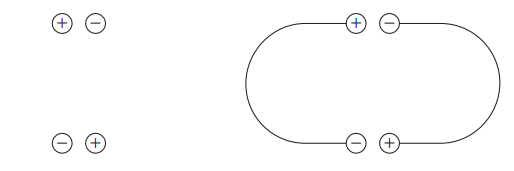
\includegraphics[width=10cm]{Electrodynamics/images/fig3.7-8.PNG}
\end{center}

\begin{proof}
Why will current flow? Well, we have a situation where the \textit{total} charge on each conductor is zero; therefore, there should be a unique way of distributing the charges across each conductor that generate the external electric field. \textit{One} way of doing so involves simply making the charge zero everywhere in each conductor. By the second uniqueness theorem we just proved, this is the \textit{only} way! So the charge will flow along the wires, canceling off.
\end{proof}

\section{The Method of Images}

\subsection{The Classic Image Problem}

It's time to present an incredible trick; it will almost feel like cheating.

\begin{example}
Suppose a point charge $q$ is held a distance $d$ above an infinite grounded conducting plane. What is the potential in the region above the plane?
\end{example}

\begin{proof}
First, note that the answer isn't simply $\frac{1}{4\pi\varepsilon_0}\frac{q}{\scr}$; the conducting plane actually does something since the electric field induces some negative charge on the nearby surface of the conductor, which affects the potential.

But how can we possibly determine the potential, if we don't know how much charge is induced or how it is distributed?

Let's place the infinite grounded conducting plane in the $xy$-plane, and the point charge at $(0,0,d)$ along the $z$-axis. Now, the problem is to solve Poisson's equation in the half-plane $z>0$ with a single point charge $q$ at $(0,0,d)$, subject to the boundary conditions
\begin{enumerate}
    \item $V=0$ when $z=0$ (as the conducting plane is grounded),
    \item $V\to 0$ at infinity.
\end{enumerate}
The first uniqueness theorem guarantees that there is a unique function $V$ that satisfies these boundary conditions. How can we construct such a function?

Here's the trick: consider a completely different setup, which consists of a point charge $q$ at $(0,0,d)$ and a point charge $-q$ at $(0,0,-d)$. The key point is that the half-plane $z>0$ has the same charge distribution, and the boundary conditions still hold:
\begin{enumerate}
    \item $V=0$ when $z=0$,
    \item $V\to 0$ at infinity.
\end{enumerate}
This is because the symmetric placement of a $-q$ charge ensures that the electric potential cancels along $z=0$. Therefore, the solution to $V$ in this setup, by the first uniqueness theorem, \textit{is the same} as the solution to $V$ in the first setup. Hence, the answer is
\[V(x,y,z)=\frac{q}{4\pi\varepsilon_0}\left[\frac{1}{\sqrt{x^2+y^2+(z-d)^2}}-\frac{1}{\sqrt{x^2+y^2+(z+d)^2}}\right] \qquad (z\ge 0).\]
The ``lower region" $z<0$ is still completely different, and we do not understand it using this method.
\end{proof}

\subsection{Induced Surface Charge}

\begin{example}
In the setup above, determine the surface charge $\sigma$ induced on the conductor.
\end{example}

\begin{proof}
In the most general situation, we can simply invoke the equation
\[\frac{\partial V}{\partial n}=-\frac{\sigma}{\varepsilon_0}\]
from Subsection \ref{surfcharforcond}, where $\frac{\partial V}{\partial n}=(\nabla V)\cdot\hat{n}$ is the directional derivative in the normal direction.

In the situation above, we can take
\begin{align*}
\sigma(x,y)&=-\varepsilon_0\left.\frac{\partial V}{\partial z}\right\rvert_{z=0}\\
&=-\varepsilon_0\cdot \frac{q}{4\pi\varepsilon_0}\left[\frac{d-z}{(x^2+y^2+(z-d)^2)^{3/2}}+\frac{d+z}{(x^2+y^2+(z+d)^2)^{3/2}}\right]_{z=0}\\
&=\boxed{\frac{-qd}{2\pi(x^2+y^2+d^2)^{3/2}}}.
\end{align*}
For some sanity checks, note that the induced charge is negative and greatest at $x=y=0$. For a further sanity check, we can integrate it over the plane
\begin{align*}
    \iint_{\mathbb{R}^2}\sigma(x,y)da&=\int_{\theta=0}^{2\pi}\int_{r=0}^\infty \frac{-qd}{2\pi(r^2+d^2)^{3/2}}\cdot rdrd\theta\\
    &=-q\int_{0}^\infty\frac{rd}{(r^2+d^2)^{3/2}}dr\\
    &=-q\left[\frac{d}{2}\cdot \frac{-2}{\sqrt{r^2+d^2}}\right]_0^\infty=-q,
\end{align*}
as expected.

\end{proof}

\subsection{Force and Energy}

\begin{example}
What is the force of attraction between the point charge and the plane?
\end{example}

\begin{proof}
Once again, considering the analog problem with two point charges $+q$ and $-q$ suffices, since the local potential around $+q$ is all that determines the force on it, and it is the same in both setups. Therefore, the force is simply
\[\vec{F}=-\frac{1}{4\pi\varepsilon_0}\frac{q^2}{(2d)^2}\hat{z}.\]
\end{proof}

\begin{example}
How do the energies of the two analogous setups (the point charge and plane versus the two opposite point charges) compare?
\end{example}

\begin{proof}
With two point charges, the energy is simply
\[W=-\frac{1}{4\pi\varepsilon_0}\frac{q^2}{2d}.\]
However, it turns out that for a single charge and conducting plane, the energy is \textit{half}:
\[W=-\frac{1}{4\pi\varepsilon_0}\frac{q^2}{4d}.\]
One way to figure out why is to consider the energy stored in the fields
\[W=\iiint_{\mathbb{R}^3}\frac{\varepsilon_0E^2}{2}d\tau,\]
and note that in the plane case we only have the upper region $z\ge 0$ of fields, so we should only get half the energy.

We can also compute the energy by calculating the work required to bring $q$ in from infinity.
\end{proof}

\begin{remark}
One way to conceptualize the difference between these cases is that with the plane,w e are doing work on a \textit{single} point charge to bring it in. The induced charge on the conductor is shifting around, but this costs no work since the potential is zero (you can also think of the fact that it is a conductor, so charge can move around freely).

In the analog case with two charges, however, we need to do work to pull in \textit{both} of them, so the energy stored is twice as much.
\end{remark}

\subsection{Other Image Problems}

We can apply the above technique to any collection of point charges near a grounded conducting plane by introducing the mirror image of the setup with opposite charges (notice how introducing these opposite charges ensures that the potential along where the plane should be is 0). We call this the \vocab{method of images}.

The following application of the method of images is beautiful, and relates to circle (sphere) inversion and Apollonius circles (spheres).

\begin{example}
A point charge $q$ is situated a distance $a$ from the center of a grounded conducting sphere of radius $R$. Find the potential outside the sphere.
\end{example}

\begin{proof}
\textit{Invert} (!!) the point charge $q$ about the sphere; this gives a point that is a distance 
\[b=\frac{R^2}{a}\]
away from the center, along the ray from the center of the sphere to the point charge $q$. Imbue this point charge with charge
\[q'=-\frac{R}{a}q.\]
We claim that this setup has zero potential along the surface of the sphere; this is true by Appolonius spheres. Therefore, the potential is indeed
\[\boxed{V(\vec{r})=\frac{1}{4\pi\varepsilon_0}\left(\frac{q}{\scr}+\frac{q'}{\scr'}\right)}\]
outside the sphere, where $\scr$ is the distance to $q$ and $\scr'$ is the distance to $q'$.
\end{proof}

\begin{remark}
You cannot place image charges in the region where you are calculating $V$! That would charge $\rho$, and you'd be solving Poisson's equation with incorrect $\rho$ (even if the boundary conditions are the same).
\end{remark}

\begin{example}
What is the force of attraction between the point and sphere?
\end{example}

\begin{proof}
It is simply the force between the charge and the image charge $q'$ we placed:
\[F=\frac{1}{4\pi\varepsilon_0}\frac{qq'}{(a-b)^2}=\boxed{-\frac{1}{4\pi\varepsilon_0}\frac{q^2Ra}{(a^2-R^2)^2}}.\]
\end{proof}

The method of images is incredibly simple and magical. It comes down to figuring out the correct ``auxiliary" configuration of image charges to make sure the grounded conductors in the setup have potential zero. However, for most shapes, this is forbiddingly complicated, if not impossible. So use with care!


